\documentclass[12pt,letterpaper]{article}\usepackage[]{graphicx}\usepackage[]{color}
%% maxwidth is the original width if it is less than linewidth
%% otherwise use linewidth (to make sure the graphics do not exceed the margin)
\makeatletter
\def\maxwidth{ %
  \ifdim\Gin@nat@width>\linewidth
    \linewidth
  \else
    \Gin@nat@width
  \fi
}
\makeatother

\definecolor{fgcolor}{rgb}{0.345, 0.345, 0.345}
\newcommand{\hlnum}[1]{\textcolor[rgb]{0.686,0.059,0.569}{#1}}%
\newcommand{\hlstr}[1]{\textcolor[rgb]{0.192,0.494,0.8}{#1}}%
\newcommand{\hlcom}[1]{\textcolor[rgb]{0.678,0.584,0.686}{\textit{#1}}}%
\newcommand{\hlopt}[1]{\textcolor[rgb]{0,0,0}{#1}}%
\newcommand{\hlstd}[1]{\textcolor[rgb]{0.345,0.345,0.345}{#1}}%
\newcommand{\hlkwa}[1]{\textcolor[rgb]{0.161,0.373,0.58}{\textbf{#1}}}%
\newcommand{\hlkwb}[1]{\textcolor[rgb]{0.69,0.353,0.396}{#1}}%
\newcommand{\hlkwc}[1]{\textcolor[rgb]{0.333,0.667,0.333}{#1}}%
\newcommand{\hlkwd}[1]{\textcolor[rgb]{0.737,0.353,0.396}{\textbf{#1}}}%

\usepackage{framed}
\makeatletter
\newenvironment{kframe}{%
 \def\at@end@of@kframe{}%
 \ifinner\ifhmode%
  \def\at@end@of@kframe{\end{minipage}}%
  \begin{minipage}{\columnwidth}%
 \fi\fi%
 \def\FrameCommand##1{\hskip\@totalleftmargin \hskip-\fboxsep
 \colorbox{shadecolor}{##1}\hskip-\fboxsep
     % There is no \\@totalrightmargin, so:
     \hskip-\linewidth \hskip-\@totalleftmargin \hskip\columnwidth}%
 \MakeFramed {\advance\hsize-\width
   \@totalleftmargin\z@ \linewidth\hsize
   \@setminipage}}%
 {\par\unskip\endMakeFramed%
 \at@end@of@kframe}
\makeatother

\definecolor{shadecolor}{rgb}{.97, .97, .97}
\definecolor{messagecolor}{rgb}{0, 0, 0}
\definecolor{warningcolor}{rgb}{1, 0, 1}
\definecolor{errorcolor}{rgb}{1, 0, 0}
\newenvironment{knitrout}{}{} % an empty environment to be redefined in TeX

\usepackage{alltt}
 \usepackage[left=2cm,right=2cm,top=2cm,bottom=2cm]{geometry}
\usepackage[ansinew]{inputenc}
\usepackage[spanish]{babel}
\usepackage{amsmath}
\usepackage{amsfonts}
\usepackage{amssymb}
\usepackage{dsfont}
\usepackage{multicol} 
\usepackage{subfigure}
\usepackage{graphicx}
\usepackage{float} 
\usepackage{verbatim} 
\usepackage[left=2cm,right=2cm,top=2cm,bottom=2cm]{geometry}
\usepackage{fancyhdr}
\pagestyle{fancy} 
\fancyhead[LO]{\leftmark}
\usepackage{caption}
\newtheorem{definicion}{Definci\'on}
\IfFileExists{upquote.sty}{\usepackage{upquote}}{}
\begin{document}

\begin{titlepage}
\setlength{\unitlength}{1 cm} %Especificar unidad de trabajo

\begin{center}
\textbf{{\large UNIVERSIDAD DE EL SALVADOR}\\
{\large FACULTAD MULTIDISCIPLINARIA DE OCCIDENTE}\\
{\large DEPARTAMENTO DE MATEM\'ATICA}}\\[0.50 cm]

\begin{picture}(18,4)
 \put(7,0){
\includegraphics[width=4cm]{minerva.jpg}}
\end{picture}
\\[0.25 cm]

\textbf{{\large Licenciatura en Estad\'istica}\\[1.25cm]
{\large Control Estad\'istico del Paquete R }\\[2 cm]
%\setlength{\unitlength}{1 cm}
{\large  \textbf{''UNIDAD UNO"}}\\[3 cm]
{\large Alumna:}\\
{\large Erika Beatr\'iz Guill\'en Pineda}\\[2cm]
{\large Fecha de elaboraci\'on}\\
Santa Ana - \today }
\end{center}
\end{titlepage}

\newtheorem{teorema}{Teorema}
\newtheorem{prop}{Proposici\'on}[section]

\lhead{Pr\'actica 05}

\lfoot{LICENCIATURA EN ESTAD\'ISTICA}
\cfoot{UESOCC}
\rfoot{\thepage}
%\pagestyle{fancy} 

\setcounter{page}{1}
\newpage

\section {ESTRUCTURA CONDICIONAL: LA ORDEN IF() Y IFELSE()}
\begin{itemize}
\item Por ejemplo, ejecute las siguientes instrucciones
\end {itemize}
\begin{knitrout}
\definecolor{shadecolor}{rgb}{0.969, 0.969, 0.969}\color{fgcolor}\begin{kframe}
\begin{alltt}
\hlstd{x} \hlkwb{<-} \hlkwd{c}\hlstd{(}\hlnum{6}\hlopt{:-}\hlnum{4}\hlstd{);}
\hlstd{x}
\end{alltt}
\begin{verbatim}
##  [1]  6  5  4  3  2  1  0 -1 -2 -3 -4
\end{verbatim}
\begin{alltt}
\hlkwd{sqrt}\hlstd{(x)} \hlcom{# Produce un mensaje de advertencia}
\end{alltt}


{\ttfamily\noindent\color{warningcolor}{\#\# Warning in sqrt(x): Se han producido NaNs}}\begin{verbatim}
##  [1] 2.449490 2.236068 2.000000 1.732051 1.414214 1.000000 0.000000
##  [8]      NaN      NaN      NaN      NaN
\end{verbatim}
\begin{alltt}
\hlkwd{sqrt}\hlstd{(}\hlkwd{ifelse}\hlstd{(x} \hlopt{>=} \hlnum{0}\hlstd{, x,} \hlnum{NA}\hlstd{))} \hlcom{# No produce advertencia}
\end{alltt}
\begin{verbatim}
##  [1] 2.449490 2.236068 2.000000 1.732051 1.414214 1.000000 0.000000
##  [8]       NA       NA       NA       NA
\end{verbatim}
\begin{alltt}
\hlkwd{ifelse}\hlstd{(x} \hlopt{>=} \hlnum{0}\hlstd{,} \hlkwd{sqrt}\hlstd{(x),} \hlnum{NA}\hlstd{)} \hlcom{# Produce un mensaje de advertencia}
\end{alltt}


{\ttfamily\noindent\color{warningcolor}{\#\# Warning in sqrt(x): Se han producido NaNs}}\begin{verbatim}
##  [1] 2.449490 2.236068 2.000000 1.732051 1.414214 1.000000 0.000000
##  [8]       NA       NA       NA       NA
\end{verbatim}
\begin{alltt}
\hlcom{# Comente las diferencias entre cada una de las instrucciones anteriores.}
\end{alltt}
\end{kframe}
\end{knitrout}
\newpage
\section {ESTRUCTURAS ITERATIVAS O DE REPETICI\'ON: FOR(), WHILE() Y REPEAT()}
\begin{itemize}
\item Ejemplo:
\end {itemize}
\begin{knitrout}
\definecolor{shadecolor}{rgb}{0.969, 0.969, 0.969}\color{fgcolor}\begin{kframe}
\begin{alltt}
\hlstd{x} \hlkwb{<-} \hlkwd{c}\hlstd{(}\hlnum{2}\hlstd{,} \hlnum{6}\hlstd{,} \hlnum{4}\hlstd{,} \hlnum{7}\hlstd{,} \hlnum{5}\hlstd{,} \hlnum{1}\hlstd{)}
\hlstd{suma}\hlkwb{<-}\hlnum{0}\hlstd{;} \hlkwa{for}\hlstd{(i} \hlkwa{in} \hlnum{1}\hlopt{:}\hlnum{3}\hlstd{) suma} \hlkwb{=} \hlstd{suma}\hlopt{+}\hlstd{x[i]; suma}
\end{alltt}
\begin{verbatim}
## [1] 12
\end{verbatim}
\end{kframe}
\end{knitrout}


\section {FUNCIONES ESCRITAS POR EL USUARIO}
\begin {itemize}
\item Ejemplo 1: Definir en R la funci\'on cuadr\'atica y = f ( x) = (3x^2) - (5x) + 2
\end {itemize}
\begin{knitrout}
\definecolor{shadecolor}{rgb}{0.969, 0.969, 0.969}\color{fgcolor}\begin{kframe}
\begin{alltt}
\hlstd{func.cuadratica} \hlkwb{<-} \hlkwa{function}\hlstd{(}\hlkwc{x}\hlstd{)}
\hlstd{\{}
\hlnum{3}\hlopt{*}\hlstd{x}\hlopt{^}\hlnum{2}\hlopt{-}\hlnum{5}\hlopt{*}\hlstd{x}\hlopt{+}\hlnum{2}
\hlstd{\}}
\hlstd{y} \hlkwb{<-} \hlkwd{func.cuadratica}\hlstd{(}\hlnum{2}\hlstd{);y}
\end{alltt}
\begin{verbatim}
## [1] 4
\end{verbatim}
\end{kframe}
\end{knitrout}
\textbf{NOTA: Toda funci\'on para usarla debe estar cargada en el \'area de trabajo (Workspace). Es decir, primero es necesario correr el c\'odigo necesario el c\'odigo de la funci\'on y asegurarse que no contenga errores de sintaxis.}
\begin{itemize}
\item Ejemplo 2: Se quiere definir una funci\'on para calcular la media de un vector de datos
\end {itemize}
Una definici\'on podr\'ia ser:
\begin{knitrout}
\definecolor{shadecolor}{rgb}{0.969, 0.969, 0.969}\color{fgcolor}\begin{kframe}
\begin{alltt}
\hlstd{media} \hlkwb{<-} \hlkwa{function}\hlstd{(}\hlkwc{x}\hlstd{)}
\hlstd{\{}

  \hlstd{n} \hlkwb{=} \hlkwd{length}\hlstd{(x)}
\hlstd{suma} \hlkwb{<-} \hlnum{0.0}
\hlkwa{for}\hlstd{(i} \hlkwa{in} \hlnum{1}\hlopt{:}\hlstd{n) suma} \hlkwb{=} \hlstd{suma} \hlopt{+} \hlstd{x[i]}
\hlstd{media} \hlkwb{=} \hlstd{suma}\hlopt{/}\hlstd{n}

\hlstd{\}}
\hlkwd{save}\hlstd{(media,} \hlkwc{file}\hlstd{=} \hlstr{"media.RData"}\hlstd{)}
\hlkwd{rm}\hlstd{(}\hlkwc{list}\hlstd{=}\hlkwd{ls}\hlstd{(}\hlkwc{all}\hlstd{=}\hlnum{TRUE}\hlstd{))}
\hlkwd{load}\hlstd{(}\hlstr{"media.RData"}\hlstd{)}

\hlstd{x} \hlkwb{<-} \hlnum{1}\hlopt{:}\hlnum{5}\hlstd{;}
\hlstd{(}\hlkwd{media}\hlstd{(x))} \hlcom{# Se usa doble par\textbackslash{}'entesis para que muestre el resultado en pantalla}
\end{alltt}
\begin{verbatim}
## [1] 3
\end{verbatim}
\begin{alltt}
\hlstd{y} \hlkwb{<-} \hlkwd{c}\hlstd{(}\hlnum{5}\hlstd{,} \hlnum{NA} \hlstd{,} \hlnum{4}\hlstd{,} \hlnum{9}\hlstd{);}
\hlstd{(}\hlkwd{media}\hlstd{(y))} \hlcom{# El resultado no puede calcularse pues falta un dato}
\end{alltt}
\begin{verbatim}
## [1] NA
\end{verbatim}
\begin{alltt}
\hlstd{z} \hlkwb{<-} \hlkwd{c}\hlstd{(}\hlnum{5}\hlstd{,} \hlnum{1} \hlstd{,} \hlnum{4}\hlstd{,} \hlnum{9}\hlstd{);}
\hlstd{(}\hlkwd{media}\hlstd{(z))}
\end{alltt}
\begin{verbatim}
## [1] 4.75
\end{verbatim}
\begin{alltt}
\hlstd{(media)} \hlcom{# Nos muestra el c\textbackslash{}'odigo de la funci\textbackslash{}'on}
\end{alltt}
\begin{verbatim}
## function(x)
## {
## 
##   n = length(x)
## suma <- 0.0
## for(i in 1:n) suma = suma + x[i]
## media = suma/n
## 
## }
\end{verbatim}
\end{kframe}
\end{knitrout}
\begin{itemize}
\item Ejemplo 3: Se quiere definir una funci\'on para graficar la funci\'on seno de x
\end {itemize}
Una definici\'on de esta funci\'on puede ser:
\begin{knitrout}
\definecolor{shadecolor}{rgb}{0.969, 0.969, 0.969}\color{fgcolor}\begin{kframe}
\begin{alltt}
\hlstd{Seno} \hlkwb{<-} \hlkwa{function}\hlstd{(}\hlkwc{x}\hlstd{)}
\hlstd{\{}

  \hlstd{y} \hlkwb{=} \hlkwd{sin}\hlstd{(x)}
\hlkwd{plot}\hlstd{(x, y,} \hlkwc{main}\hlstd{=}\hlstr{"Ejemplo de gr\textbackslash{}'aficos en R"}\hlstd{,}
\hlkwc{xlab}\hlstd{=}\hlstr{"x"}\hlstd{,} \hlkwc{ylab}\hlstd{=}\hlstr{"y = Seno(x)"}\hlstd{,} \hlkwc{col}\hlstd{=}\hlstr{"blue"}\hlstd{,} \hlkwc{pch}\hlstd{=}\hlnum{1}\hlstd{)}

\hlstd{\}}
\hlcom{# Pruebe la funci\textbackslash{}'on con el siguiente vector:}

\hlstd{x}\hlkwb{<-}\hlkwd{seq}\hlstd{(}\hlopt{-}\hlstd{pi, pi,} \hlkwc{len}\hlstd{=}\hlnum{100}\hlstd{)}

\hlkwd{Seno}\hlstd{(x)}
\end{alltt}
\end{kframe}
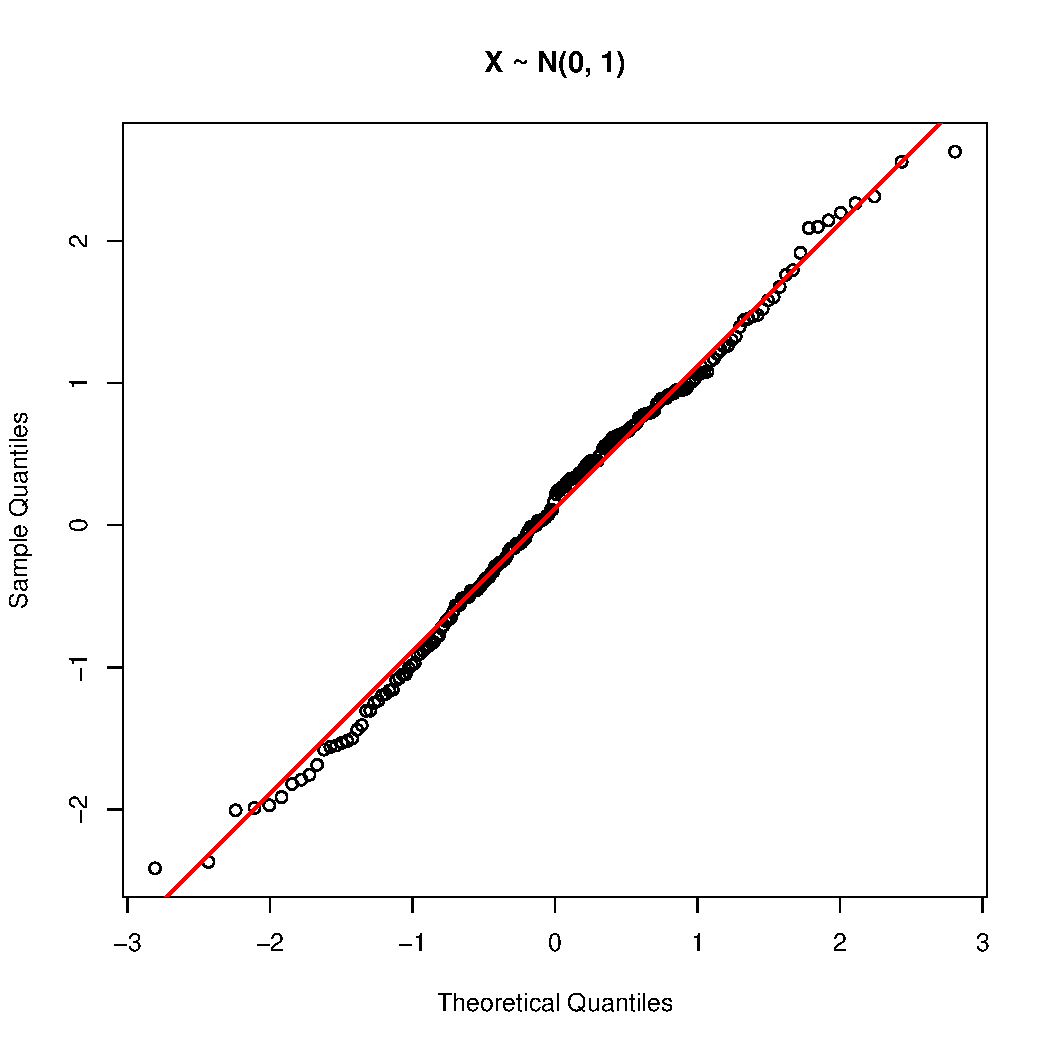
\includegraphics[width=\maxwidth]{figure/unnamed-chunk-5-1} 

\end{knitrout}
\newpage
\section{EJERCICIOS PROPUESTOS}
\begin{itemize}
\item Ejercicio 1: Escriba una funci\'on para encontrar el factorial de un n\'umero mayor que cero
\end{itemize}
\begin{knitrout}
\definecolor{shadecolor}{rgb}{0.969, 0.969, 0.969}\color{fgcolor}\begin{kframe}
\begin{alltt}
\hlstd{fac}\hlkwb{<-}\hlkwa{function}\hlstd{(}\hlkwc{f}\hlstd{)\{ prod}\hlkwb{<-}\hlnum{1} \hlcom{# Inicializar el producto en 1}
\hlkwa{if} \hlstd{(f}\hlopt{==}\hlnum{0}\hlstd{)\{} \hlcom{# Cuando el valor ingresado es cero}
  \hlstd{prod}\hlkwb{<-}\hlnum{1} \hlcom{# El factorial es 1}
  \hlkwd{return}\hlstd{(prod)}
\hlstd{\}}
  \hlkwa{else}\hlstd{\{}
    \hlkwa{if}\hlstd{(f}\hlopt{<}\hlnum{0}\hlstd{)} \hlcom{# Cuando el valor ingresado es negativo}
      \hlkwd{print}\hlstd{(}\hlstr{"No existe el factorial de un n\textbackslash{}'umero negativo"}\hlstd{)}
    \hlkwa{else} \hlstd{\{}
      \hlstd{int}\hlkwb{<-}\hlkwd{c}\hlstd{(}\hlnum{1}\hlopt{:}\hlstd{f)} \hlcom{# Cuando el valor es positivo}

      \hlkwa{for}\hlstd{(i} \hlkwa{in} \hlstd{int)}
        \hlstd{prod}\hlkwb{<-}\hlstd{prod} \hlopt{*} \hlstd{i}
      \hlkwd{return}\hlstd{(prod)}
    \hlstd{\}}
  \hlstd{\}}

  \hlstd{\}}
\hlkwd{fac}\hlstd{(}\hlnum{4}\hlstd{)}
\end{alltt}
\begin{verbatim}
## [1] 24
\end{verbatim}
\end{kframe}
\end{knitrout}
\begin{itemize}
\item Ejercicio 2: Escriba una funci\'on para encontrar la varianza o la cuasi-varianza de un vector de
datos.
\end{itemize}
\begin{knitrout}
\definecolor{shadecolor}{rgb}{0.969, 0.969, 0.969}\color{fgcolor}\begin{kframe}
\begin{alltt}
\hlstd{vx}\hlkwb{<-}\hlkwa{function}\hlstd{(}\hlkwc{k}\hlstd{) \{ suma} \hlkwb{<-} \hlnum{0.0}
  \hlstd{z}\hlkwb{<-}\hlkwd{length}\hlstd{(k)}
  \hlkwa{for}\hlstd{(i} \hlkwa{in} \hlnum{1}\hlopt{:}\hlstd{z)\{}
    \hlstd{suma} \hlkwb{=} \hlstd{suma} \hlopt{+} \hlstd{k[i]}
    \hlstd{media} \hlkwb{=} \hlstd{suma}\hlopt{/}\hlstd{z} \hlcom{# Obtener la media aritmetica del vector}
    \hlkwa{for}\hlstd{(i} \hlkwa{in} \hlnum{1}\hlopt{:}\hlstd{z)\{}
      \hlstd{vx}\hlkwb{<-}\hlstd{k[i]}\hlopt{-}\hlstd{media}
      \hlstd{vx}\hlkwb{<-}\hlstd{(vx)}\hlopt{/}\hlstd{z}
    \hlstd{\}}
  \hlstd{\}}
  \hlkwd{return}\hlstd{(vx)}
\hlstd{\}}
\hlstd{k} \hlkwb{<-} \hlkwd{c}\hlstd{(}\hlnum{2}\hlstd{,}\hlnum{3}\hlstd{,}\hlnum{4}\hlstd{)}
\hlstd{(}\hlkwd{vx}\hlstd{(k))}
\end{alltt}
\begin{verbatim}
## [1] 0.3333333
\end{verbatim}
\end{kframe}
\end{knitrout}
\begin{itemize}
\item Ejercicio 3: Escriba una funci\'on para encontrar la media geom\'etrica de un vector de datos
\end{itemize}
\begin{knitrout}
\definecolor{shadecolor}{rgb}{0.969, 0.969, 0.969}\color{fgcolor}\begin{kframe}
\begin{alltt}
\hlcom{# Obtener la ra?z n-esima de cualquier valor }
\hlstd{raiz}\hlkwb{=}\hlkwa{function}\hlstd{(}\hlkwc{m}\hlstd{,}\hlkwc{n}\hlstd{)\{} \hlcom{# Este es la funci\textbackslash{}'on que llamamos en los dos c\textbackslash{}'odigos siguientes}
  \hlstd{raiz}\hlkwb{=}\hlstd{n}\hlopt{^}\hlstd{(}\hlnum{1}\hlopt{/}\hlstd{m)}
  \hlkwd{return}\hlstd{(raiz)}
\hlstd{\}}
\hlkwd{raiz}\hlstd{(}\hlnum{3}\hlstd{,}\hlnum{27}\hlstd{)}
\end{alltt}
\begin{verbatim}
## [1] 3
\end{verbatim}
\begin{alltt}
\hlcom{# Caso cuando el vector esta ordenado, es decir desde 1 hasta el valor deseado}
\hlstd{MG}\hlkwb{<-}\hlkwa{function}\hlstd{(}\hlkwc{m}\hlstd{)}
  \hlstd{\{prod}\hlkwb{<-}\hlnum{1} \hlcom{# Este c\textbackslash{}'odigo se parece al del factorial de un numero positivo}
  \hlstd{int}\hlkwb{<-}\hlkwd{c}\hlstd{(}\hlnum{1}\hlopt{:}\hlstd{m)}

  \hlkwa{for}\hlstd{(i} \hlkwa{in} \hlstd{int)}
    \hlstd{prod}\hlkwb{<-}\hlstd{prod} \hlopt{*} \hlstd{i}
  \hlstd{raiz}\hlkwb{=}\hlkwd{raiz}\hlstd{(m,prod)}
  \hlcom{# Obtener la ra\textbackslash{}'iz n-esima (corresponde a la cantidad de valores en el vector)}
  \hlkwd{return}\hlstd{(raiz)}
  \hlstd{\}}
\hlkwd{MG}\hlstd{(}\hlnum{5}\hlstd{)}
\end{alltt}
\begin{verbatim}
## [1] 2.605171
\end{verbatim}
\begin{alltt}
\hlcom{# Caso cuando el vector es de calquier forma que el usuario desee}
\hlstd{MG2}\hlkwb{<-}\hlkwa{function}\hlstd{(}\hlkwc{g}\hlstd{) \{product}\hlkwb{<-}\hlnum{1} \hlcom{# Inicializar el producto}
  \hlstd{p}\hlkwb{<-} \hlkwd{length}\hlstd{(g)} \hlcom{# Guardar la longitud del vector}
  \hlkwa{for}\hlstd{(i} \hlkwa{in} \hlnum{1}\hlopt{:}\hlstd{p)}
    \hlstd{product}\hlkwb{<-}\hlstd{product} \hlopt{*} \hlstd{g[i]} \hlcom{# Realizar el producto de cada valor del vector}
  \hlstd{MG2}\hlkwb{<-}\hlstd{product} \hlcom{# Guardar el producto en MG2}
  \hlstd{raiz}\hlkwb{<-}\hlkwd{raiz}\hlstd{(}\hlkwd{length}\hlstd{(g),MG2)}
  \hlcom{# Obtener la raiz n-esima (corresponde a la cantidad de valores en el vector)}
  \hlkwd{return}\hlstd{(raiz)}
\hlstd{\}}
\hlstd{g}\hlkwb{<-}\hlkwd{c}\hlstd{(}\hlnum{2}\hlstd{,}\hlnum{3}\hlstd{,}\hlnum{4}\hlstd{,}\hlnum{5}\hlstd{)} \hlcom{# Pasar el vector de datos}
\hlstd{(}\hlkwd{MG2}\hlstd{(g))}
\end{alltt}
\begin{verbatim}
## [1] 3.309751
\end{verbatim}
\end{kframe}
\end{knitrout}
\newpage
\begin{itemize}
\item Ejercicio 4: Escriba una funci\'on para encontrar la media arm?nica de un vector de datos
\end{itemize}
\begin{knitrout}
\definecolor{shadecolor}{rgb}{0.969, 0.969, 0.969}\color{fgcolor}\begin{kframe}
\begin{alltt}
\hlstd{MA} \hlkwb{<-} \hlkwa{function}\hlstd{(}\hlkwc{x}\hlstd{)}
  \hlstd{\{suma} \hlkwb{<-} \hlnum{0.0} \hlcom{# Inicializar suma}
  \hlstd{n} \hlkwb{<-} \hlkwd{length}\hlstd{(x)} \hlcom{# Guardar la longitud del vector}
  \hlkwa{for}\hlstd{(i} \hlkwa{in} \hlnum{1}\hlopt{:}\hlstd{n)}
    \hlstd{suma} \hlkwb{<-} \hlstd{suma} \hlopt{+} \hlstd{(}\hlnum{1}\hlopt{/}\hlstd{x[i])}
  \hlcom{# Realizar la suma, pero de los reciprocos (1/x[i]) de los valores del vector}
  \hlstd{denom} \hlkwb{<-} \hlstd{suma}\hlopt{/}\hlstd{n} \hlcom{# Encontrar la media de los reciprocos}
  \hlstd{MA}\hlkwb{<-}\hlnum{1}\hlopt{/}\hlstd{denom}

\hlstd{\}}
\hlstd{x} \hlkwb{<-} \hlkwd{c}\hlstd{(}\hlnum{2}\hlstd{,}\hlnum{3}\hlstd{)}
\hlcom{# Pasar el vector de datos}
\hlstd{(}\hlkwd{MA}\hlstd{(x))}
\end{alltt}
\begin{verbatim}
## [1] 2.4
\end{verbatim}
\end{kframe}
\end{knitrout}


\end{document}
